% Template Created by Albert Alises Sorribas (albert.alises@gmail.com) for the thesis of the MSc. in Computational Biomedical Engineering, Universitat Pompeu Fabra. Based on the thesis template of the Imperial College London,  downloadable at http://www.imperial.ac.uk/brand-style-guide/templates/downloadable-templates/

\documentclass[a4paper,12pt,twoside]{report}
\usepackage[left=3cm,right=3cm,top=3cm,bottom=3cm]{geometry} %Margins
\usepackage{pdfpages}
\usepackage{hyperref}
\usepackage{listings}
\usepackage{xcolor}
\usepackage{setspace}
\usepackage{tocloft}
\usepackage{amsmath}
\usepackage{chngcntr }
\usepackage{multirow}
\usepackage[toc,page]{appendix}
\usepackage[T1]{fontenc}
\usepackage[nottoc]{tocbibind}
\usepackage[compact]{titlesec}
\usepackage[nameinlink,capitalise]{cleveref}
\titlespacing{\section}{0pt}{1ex}{0ex}
\titlespacing{\subsection}{0pt}{1ex}{0ex}
\titlespacing{\subsubsection}{0pt}{1ex}{0ex}

\counterwithout{figure}{chapter}
\counterwithout{table}{chapter}

\include{thesis.preamble}

\begin{document}

\newgeometry{left=2cm,right=2cm} %Only for the title new margins

%Title parameters
\title{Automatic harmonic analysis of classical string quartets from symbolic score}
\author{N\'estor N\'apoles L\'opez}
\submitdate{September 2017}
\supervisor{Xavier Serra}
\cosupervisor{Rafael Caro}

\maketitle

\maketitle
\restoregeometry

\preface
\cleardoublepage
%\addcontentsline{toc}{chapter}{Acknowledgement}
\begin{dedication}
\pagenumbering{gobble}% Remove page numbers (and reset to 1)

Grandmother, Juan Rodrigo Perez Cardenas. Family. Kinga.

\newpage

\end{dedication}

%\addcontentsline{toc}{chapter}{Acknowledgement}

\begin{acknowledgement}
\pagenumbering{gobble}% Remove page numbers (and reset to 1)

Xavier Serra, I am thankful for the trust deposited in my music theory skills for performing this work, and for allowing me to contribute to the CompMusic project.

Rafael Caro, thank you for helping with the harmonic analyses and the fast review of every presentation and thesis draft.

Craig Sapp, thank you for the fast response in the topics related to Humdrum Extras, the Verovio Humdrum Viewer and for pointing out to relevant research I was unaware of. 

\newpage
\end{acknowledgement}

%\addcontentsline{toc}{chapter}{Abstract}

\begin{abstract}
\pagenumbering{gobble}

This work proposes running an automatic harmonic analysis over a novell dataset of String Quartets from Joseph Haydn. Using implementation code from David Temperley, Daniel Sleator and Craig Sapp. Additionally, proposes an evaluation method to measure the similarity of the resulting analyses against manual annotations included in the String Quartet dataset. 24 musical scores analyzed and evaluated with a range of 15\% to 85\% accuracy for the Temperley algorithm.

\bigskip
Keywords: Automatic harmonic analysis; Joseph Haydn; String quartet; Roman numeral analysis


\newpage
\end{abstract}


\body

\normallinespacing

% Introduction of the project
\chapter{Introduction}
In the traditional sense, harmonic analysis relates to a set of music theory studies that pretend to describe the relationship of simultaneous sonorities and generalize rules of how each of the voices involved should move to facilitate and embellish these simultaneous sonorities.

It is difficult, however, to give a precise definition of where the task of harmonic analysis starts and finishes. As will be discussed in the literature review, different researchers have made different characterizations of the problem, sometimes binding these characterizations closely to the mathematical tools they have used to approach the problem, in other cases to the type of music that they pretend to analyze, and in other cases, it could be due to other circumstances. For this particular work, I intend to define harmonic analysis based in two simple definitions, and afterwards, the outcome definition will help to describe which are the expected inputs and outputs of an automatic harmonic analysis system.

\section{Automatic harmonic analysis}
According to the Oxford Music Online dictionary, the term analysis could be defined as the following: \cite{oxfordanalysis}

\begin{quote}
\centering
\emph{[...] the interpretation of structures in music, \linebreak
their resolution into relatively simpler constituent elements, \linebreak and the investigation of the relevant functions of those elements.}
\end{quote}

Additionally, according to the same source, a very simplistic definition of harmony could be: \cite{oxfordharmony}

\begin{quote}
\centering
\emph{The simultaneous sounding (i.e. combination) of notes [...]}
\end{quote}

Combining these definitions, one possible interpretation of what is a harmonic analysis could be the following:

\begin{quote}
\centering
\emph{[...] the interpretation of \textbf{harmonic} structures in music, \linebreak
their resolution into relatively simpler \textbf{harmonic labels}, \linebreak and the investigation of the relevant functions of those \textbf{labels}.}
\end{quote}

Therefore, as stated by this definition, the process of harmonic analysis comprises three steps:

\begin{itemize}
  \item Interpreting the harmonic structures in music
  \item Resolving these harmonic structures into harmonic labels
  \item Investigating the relevant functions among these labels
\end{itemize}

For breaking down the steps of the analysis, we could use a fragment of a musical score.

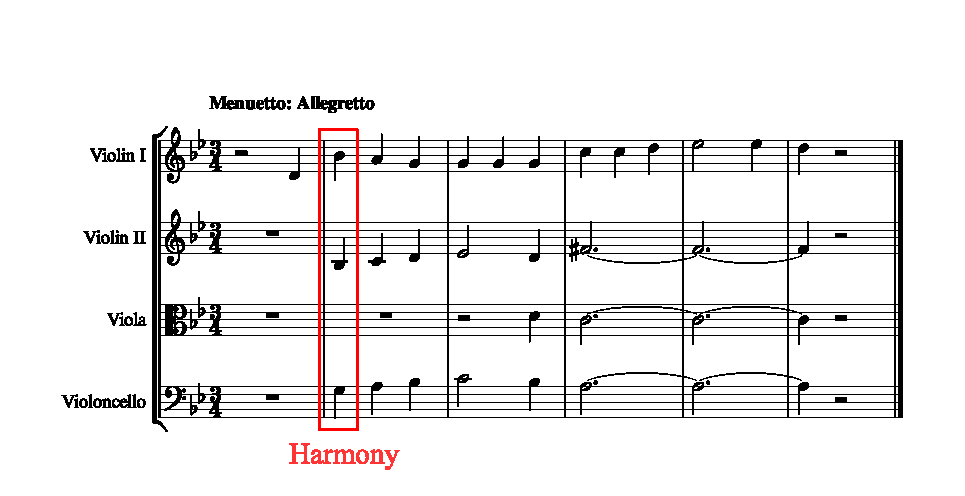
\includegraphics{figures/1}

\section{Motivation}
The main reason why it would be benefical for musicians and musicologists to automate a harmonic analysis is because it takes a considerable amount of time and knowledge to perform these analyses. In practice, students at conservatoires often learn the guidelines of harmonic analysis during a specialized course of Harmony. Such a course could extend to several years, making it a difficult discipline to learn fast for a beginner. Even in the case of experts, it might take relatively long time to analyze a piece of music in terms of harmony, which makes the task of automating it valuable even for the expert theorist.

\section{Objectives}
This work pretends to reproduce and apply the current approach for automatic functional harmonic analysis used over the KernScores corpora, and apply it to a specific set of string quartets from Joseph Haydn. Once these automatic analyses are performed, they will be compared to manual annotations over the same set of string quartets.

\section{Structure of the Report}
Literature. Methods. Results. Discussion.

\newpage


% Description of the dataset
\chapter{Dataset}
\label{chap:dataset}
The dataset used for this work is a novell dataset created as part of the final output of this work. It consists of 24 musical scores corresponding to six string quartets, Op.20, written by Joseph Haydn. These quartets are commonly known as the \emph{Sun quartets}. The dataset lies in the following repository \url{https://github.com/napulen/haydn_op20_harm}.

\section{String quartet}

\section{Joseph Haydn}

\section{Op.20 String quartets}

\newpage


% Literature review
\chapter{Literature review}
\label{chap:literature-review}
During \autoref{chap:introduction}, I defined what a system for automatic harmonic analysis consists of, i.e., \emph{A piece of software that given a fragment of music as input, will output the same piece of music, with roman numeral labels appended to it}. At least for this particular work.

I also established during \autoref{chap:dataset} that the musical scores used for this work are encoded using the \emph{Humdrum} \cite{humdrum} grammar and the roman numerals labeled using the \emph{**harm} \cite{harm} syntax. In  this chapter, I will go through a chronological list of attempts in conceiving a system of automatic harmonic analysis.

Aftwards, I will narrow the list of attemtps, favoring the ones that could work with a musical score encoded in the humdrum grammar as input, and which can output a similar encoding with an appended **harm spine for the roman numeral labels.

Finally, I will discuss the selected attempt and the reason of its preference over other similarly suitable attempts.

% \section{Roman numerals}
% The most important argument for defending roman numerals as the chosen way to label harmonic structures, is probably the theory that one of the most verbose ways of labeling harmonic structures
%
% Harmonic analysis could be seen from different perspectives, the first one I would like to address is how it was conceived and modeled by music theorists. Starting with the french composer Jean-Philippe Rameau (1683-1764), until the theory from the german theorist Hugo Riemann (1849-1919) in the late nineteenth century.
%   \subsection{Fundamental bass}
%   The original idea by Rameau was based on the movement of the bass note, the so called \emph{Fundamental Bass}, which constructed rules and principles of how the movement of a bass note determined also the movement of the harmony. Rameau's theory limited the dictionary of chords to triads and some special cases of seventh chords, and considered chord inversions for the first time, from which the core concept of harmonic root arises and suggests that the bass note could be serving a harmonic root located in the superior voices. This theory is pioneer in separating the melodic movement and coincidence in time from counterpoint \cite{beach1974origins}, and looking at the music from a vertical perspective, a vision that spread in the following periods of western art music.
%   \subsection{Root succession tables}
%   These set of theories, denomined by Tymoczko as \emph{scale-degree} theories \cite{tymoczko2001root}, assign a number to each of the degrees in a scale, which represents its triad, and then trying to infer the most common succession of that particular scale degree to another. This theories have been used commonly in Harmony text books, and in principle, the scale-degree transitions have not been obtained scientifically. However, due to the probabilistic nature of these theories, there have been recent efforts in validating their statements and accuracy using computational resources, such as first-order Markov models.
%   \subsection{Functional harmony}
%   In 1893, Hugo Riemann presented his \emph{Vereinfachte Harmonielehre}, which placed together ideas and theories from himself and earlier theorists, and gave birth to what is called \emph{Functional Harmony}. The most notable, and allegedly controversial, characterization that comes from the functions theory, is the idea of categorization of chords. Functional harmony considers that chords belong to one of three tonal functions:
%   \begin{itemize}
%     \item Tonic
%     \item Subdominant
%     \item Dominant
%   \end{itemize}
%   These functions contain all individual chords, but are essentially represented by the primary triads: I, IV and V.
%   Due to this categorization of chords, functional harmony contains more information about tonal contexts and semantics, and therefore, as an analysis output becomes more interesting than fundamental bass or root succession theories.


\section{Overview of Automatic Harmonic Analysis}
    \subsection{The pioneer work by Terry Winograd}
    Researchers in the field mostly mention the approach from Terry Winograd \cite{winograd1968linguistics}, in 1968, as the pioneer work in the task of automatic harmonic analysis. This work is not only important because it is the first and pioneering work in computing a harmonic analysis, but also because it linked the computational techniques used in natural language processing to music. The model from Winograd was evaluated over music from Johann Sebastian Bach, and pretends to output a functional harmonic analysis of such pieces of music. To provide an output, it requires a preliminary hand-made conversion of the original score and turn it into a sequence of four-part perfect chords. This allowed him to process a score using his implementation in the LISP programming language, but it also means that during this pre-processing stage the non-harmonic tones are eliminated before solving the problem. In his 1997 harmonic analysis algorithm \cite{temperley1997algorithm}, David Temperley provided insight about the flaws of Winograd's model, among them he mentions the issues concercing melodic seggregation and arpeggiations.

    \subsection{Expert system from Maxwell}
    A direct successor of Winograd's approach, the model from John Maxwell, which was part of his PhD dissertation in 1984, and successively published in 1992 \cite{maxwell1992expert}, is probably the best example of the rule-based approaches towards harmonic analysis. Same as Winograd, Maxwell's target was to output a functional harmonic analysis from a music score. The model from Maxwell has fifty five rules that pretend to reduce the vertical sonorities into a chord sequence, and then deciding for key changes. Some of the rules are intuitive and basic, e.g.:

    \begin{quote}
    \centering
    \emph{"Perfect and imperfect consonant intervals constitute a consonant interval. Every other is a dissonant interval."},
    \end{quote}

     while others appear cryptic and difficult to understand, e.g.:

     \begin{quote}
     \centering
     \emph{"If the goal chord falls on a strong beat and it is a major triad or major-minor seventh, and the root movement from the pre-cadence is an ascending or descending perfect fifth or major second or a descending minor second, and when the root motion is a descending fifth, the pre-cadence is not a potential dominant, and when the root motion is an ascending fifth the pre-cadence is triadic, then the pseudo-cadence is a half cadence, and its strength increases by 10."}.
     \end{quote}

    The later rule also reveals a problem that was pointed out by future researchers, the use of arbitrary, fixed values while determining the strength of a cadence.

    Even so, the results of Maxwell's approach get really close to the outcome expected by a music theorist analyzing a music score and determining its functional harmony. This work was tested over three different movements of Johann Sebastian Bach's Six French Suites: The sarabande from Suite No.1, the menuet from Suite No.2 and the gavotte from Suite No.5. The pieces selected comprehend different problems and levels of complexity to be addressed: Four-part harmony with several non-harmonic tones, 2-voice continuous contrapuntual movement, and a varying contrapuntual texture, respectively. David Temperley listed the limitations of Winograd and Maxwell's approaches similarly, summarizing them in the following:
		\begin{itemize}
			\item Sequences of notes that are not displayed simultaneously (vertically), as arpeggiations of chords.
			\item Missing pitches in the spelling of a full chord, which can be deduced from the context.
			\item Ornamental notes. Maxwell proposes specific rules to deal with these notes, but according to Temperley, neither Maxwell's or Winograd's are good enough to correctly detect ornamental notes.
    \end{itemize}
    Maxwell's approach, in general, represents the powerful and sophisticated machinery of rule-based approaches, as well as their complexity.

    \subsection{Temperley and the Melisma Music Analyzer}
    Probably the most relevant approach in automatic harmonic analysis for this work, is the approach from David Temperley described in 1997 \cite{temperley1997algorithm}, as it was extended afterwards by his work in key estimation algorithms and which culminated in the implementation of the Melisma Music Analyzer, in conjunction with Daniel Sleator.
    Inspired by the cognitive experiments by Carol Krumhansl \cite{krumhansl2001cognitive}, the aim of Temperley is to produce an algorithm that models the human process of harmonic analysis done by a trained expert, and to take it as indicative of the analysis produced subconsciously by listeners in general.

		The traiditional functional harmonic analysis done in music theory courses uses the \emph{roman numerals} notation to segment a piece of music, labeling it with symbols indicating the relationship between each root to the current key. Temperley steps forward in the definition of the problem of harmonic analysis, decomposing the task into two subtasks: \emph{root finding} and \emph{key finding}. Temperley claims then that functional harmonic analysis could be broken down into these subtasks, focusing at first in root finding, assuming that this task can be done independently to key finding. Root finding basically consists of dividing a piece into segments and label each of them with a root.

    Once in the task of root-finding, Temperley approaches the task defining certain rules: \emph{Pitch variance rule, compatibility rule, strong-beat rule, harmonic variance rule and ornamental dissonance rule}. Together with these rules, he introduces important definitions that aid in the process of root analysis: The concepts of \emph{Tonal Pitch Class} (TPC), \emph{Center of Gravity} (COG) and the \emph{line of fifths}.

    It is difficult to follow the chronology of this approach, as the implementation of this model comes mainly in the form of the Melisma Music Analyzer, which was released in 2001, and included the key estimation algorithm and a combined mode that eventually performed the complete functional harmonic analysis. The latest mode being the core implementation of what will be used to compute automatic harmonic analysis during this work.

    \subsection{Probabilistic and statistical approaches}
    Temperley himself, after the release of the Melisma Music Analyzer, moved into the direction of probabilistic models. In his case, using a Bayesian approach that aims to provide a unified modeling of harmonic analysis, meter induction and melodic seggregation, challenging the individualization of these problems without considering the connections among them \cite{temperley2009unified}.

    Another important probabilistic approach that emerged to solve the problem of functional harmonic analysis was that of Christopher Raphael \cite{raphael2003harmonic}.
    This model from Raphael is one of the few pure-functional harmonic analysis approaches, oriented towards the analysis of common-practice music. The idea is simple and some of his assumptions simplify the parameters of the model. Some constant that remains as in previous models is the fact that it gets rid of all the pitch-spelling information and replaced for solely pitch information. This model, unlike Temperley, does not try to reconstruct the pitch spelling information back by any algorithmic means, and in the words of Raphael, it is an obvious extension to the model.

    Another quite important effort in the statistical domain includes the work from Martin Rohrmeier \cite{rohrmeier2008statistical}, who uses a heuristic method of segmentation. Analyzes distributions of single pitch-class-sets, chord classes and pitch-class-sets transitions. One of the goals of Rohrmeier was the research of \emph{syntacticality} in harmony. The final goal is to produce descriptive analyses of harmonic structure based on an empirical approach. The choice of the corpus is, similarly to others, music from Joahann Sebastian Bach. In his case, chorales, because they constitute a large and coherent set of pieces regarding style and composition technique. Rohrmeier claims that this work is pioneer in the statistical analysis of a corpus for the purpose of finding features of tonal harmony. According to the results of Rohrmeier, the most frequent occurrences of pitch-class-sets in this music are those of tonic, dominant and subdominant chords. This would be expected and helps to reinforce those scale-degree theories that describe harmonic movement with transition tables of scale degrees. The results from this research, apart from being interesting in confirming music-theory beliefs regarding common chords and transitions in tonal music, could also be replicated in a different corpus to target its particular common chords and transitions.

    \subsection{Grammar-based}
    Three years after his statistical work in Bach Chorales, Martin Rohrmeier brought back the use of grammars to study the underlying structure of musical harmony \cite{rohrmeier2011towards}, which inspired future works by other researchers in the field, specially towards analyzing jazz music. In this work, Rohrmeier claims that the structure of harmonic progressions exceeds the simplicity of a markovian transition table, and he proposes a set of phrase-structure grammar rules. For this purpose, the hierarchical analysis from the music-theory approach done by \cite{kostka1995tonal} is presented, with the belief that it can be brought to a closer formalization. Rohrmeier presents a tree representation of a chord sequence, using two principles:
    \begin{itemize}
			\item Chords have dependencies and the existence of one sometimes requires the existence of another
			\item Chords have functions, these functions can be realized by a set of chords.
		\end{itemize}
    The system comprises 27 rules for the generation of a grammar, this helps to model common-practice music as well as jazz music. The output of this algorithm is a hierarchical tree of the functions and dependencies of the chords. The level of detail from this work to model every special case of the harmonic language is remarkable, as careful attention has been put trying to comprehend distinct kinds of cadences, chords and modulations in the model.

    This work was eventually retaken and implemented by Bas de Haas \cite{de2013automatic} using chord labels as input for the system.

    As discussed previously, after I have overviewed the works in harmonic analysis, I will now narrow down the list of attempts that are most relevant to the expectations of this work. Among the most important factors that lead to separate the \emph{favorite} attempts from the rest, I could list two: The first one, being the capability of the system to deal with full scores as input, instead of a list of chord labels. The second, being the capability of the system to exploit, infer or reconstruct the pitch-spelling information from the original score in the output of the analyzed score.

  \section{Narrowing down the approaches}
  From the previously mentioned efforts of harmonic analysis, those that fit the best with the expected inputs and outputs of this work, are the following:
  \begin{table}[tbp]
    \centering
    \begin{tabular}{llll}
      Approach & Year & Implementation & Availability \\
      Winograd & 1968 & LISP & No \\
      Maxwell & 1992 & LISP & No \\
      Temperley & 1997\footnote{The span of time between this approach was presented as a paper and the current implentation used for this work, is much wider, reaching changes in code done during 2017} & C & Yes \\
      Raphael & 2003 & C & Partial \\
      Illescas & 2008 & Java & Partial
    \end{tabular}
    \caption{Automatic functional harmonic analysis approaches}
    \label{table:shortlist_models
  \end{table}

  From the approaches shown in \autoref{table:shortlist_models}, I decided to choose the model and implementation from David Temperley's algorithm to be run over the dataset of String Quartets Op.20.

  The most important reason for this selection is because this is the approach with the most mature implementation, and the effort for getting humdrum scores to be analyzed using it is the minimum of all the other attemtps.




\newpage


% Methodology
\normallinespacing

\chapter{Methodology}
\label{chap:methodology}

As I described during \autoref{chap:literature-review}, the original model from David Temperley divided a system of automatic harmonic analysis in two subsystems: One that performs root detection and another one that performs key detection. Thanks to the work that has been already done by David Temperley, Daniel Sleator and Craig Sapp, the idea of using an implemented model of this automatic harmonic analysis system over the dataset described in this work is already feasible by putting together different programs and scripts.

During this chapter I will go through the process of listing and joining together all the programs that are necessary to perform the automatic harmonic analysis of a humdrum musical score. I will start from the analysis programs of the Melisma Music Analyzer, which are the core of the analysis, to the scripts and programs of the Humdrum Extras software tools that allow for the use of real Humdrum music scores.

\section{The Melisma Music Analyzer}
  The Melisma Music Analyzer was implemented by Daniel Sleator over the work of David Temperley. It takes as input a "NoteFile" which is similar to a plain-text representation of midi files.
  In order to achieve a full harmonic analysis, a NoteFile needs to go through 3 stand-alone programs

  \begin{figure}[ht]
    \centering
      
\includegraphics[width=0.5\textwidth]{04-methodology/figures/1}
    \caption{Harmonic analysis as divided by David Temperley}
    \label{fig:software_stack1}
  \end{figure}

  \begin{figure}[ht]
    \centering
      
\includegraphics[width=1.0\textwidth]{04-methodology/figures/2}
    \caption{Melisma Music Analyzer, from a Notefile to a plain-text analysis}
    \label{fig:software_stack2}
  \end{figure}

  \begin{figure}[ht]
    \centering
      
\includegraphics[width=1.0\textwidth]{04-methodology/figures/3}
    \caption{Automatic harmonic analysis of a humdrum musical score}
    \label{fig:software_stack3}
  \end{figure}

  \subsection{Meter}
    This program extracts metrical information about the musical piece, using the theories of the Generative Theory of Tonal Music as a basis.
    The output of this program is the same notefile with beat information appended at the end.
  \subsection{Harmony}
    This program takes as input the notefile with beat information (the output from the meter program), and outputs information about harmonic roots for each beat. The name is somehow misleading, as this program's output is not harmony, but a harmonic root. Temperley divided the task of harmonic analysis in root estimation and key estimation, this program computing the first of these subtasks. One argument of why they decided to call it "harmony" program instead of "harmonic-root" could be that it was developed before than the key algorithm, and at that moment it was the only analysis done. This information has not been corroborated by me.
  \subsection{Key}
    This program takes as input the notefile with beat and harmonic-root information (the ouput from the harmony program). Something to remark about this program is that it might work without the information from the harmony program, estimating only the key, without using any harmonic root information. This could be seen in the following way, if David Temperley divides the problem of harmonic analysis into two subproblems: Root estimation and Key estimation, the first mode of this program pretends to solve the second problem, while in the second mode, adding the output from the "harmony" program as input, pretends to solve both subtasks and output a full harmonic analysis. The difference between these different modes relies on the user setting a certain value in the corresponding parameter file.
  \subsection{Parameter files}
    Every program from the Melisma Music Analyzer accepts a parameter file for configuring different options, such as verbosity or roman numeral analysis.
\section{Humdrum extras}
  The humdrum extras are a set of tools developed in C++ by Craig Sapp to process humdrum files (or to convert other formats into humdrum). For this work, we are particularly interested in a few of these utilities that help to process a humdrum file, pass it to the melisma music analyzer, and then bring the output back to humdrum.
  \subsubsection{Issues with Melisma's input}
    The input format from the Melisma Music Analyzer, yet it resembles a MIDI file, it is not a midi file, and it needs parsing. Humdrum extras provides a parser to convert a humdrum file into the notefile format used by Melisma, this program is called kern2melisma, and it is the first step in the workflow of a functional harmonic analysis from a humdrum score.
  \subsubsection{Piping the output key to key2humdrum}
    Once the file is in Melisma's format, it can go through the melisma programs, as the output of these programs becomes the input for the next one, the files can be piped in unix environment, so it looks like this: kern2melisma | meter | harmony | key.
    At this point, we have the output of the key program from Melisma, this outputs needs additional processing to go back into a humdrum file. There are two programs from Craig Sapp of the MuseInfo tools that enable this process. In this work, I am requiring mainly the key2humdrum program, as this is the one taking the input from the key program, optionally parsing the roman numerals included with the output of the key program.
  \subsubsection{Appending to a humdrum file}
    The last step in getting the information back into a humdrum file is parsing the output of the key2melisma program and appending this information to a humdrum spine. This process is not done by a standalone program, but rather a program that comprehends all the process described before.
  \subsubsection{tsroot summarizes everything}
    The tsroot programs performs all the steps described before, plus interpreting the output of key2humdrum and producing a final humdrum score with the analysis information appended to it.
\section{KernScores}
  \subsection{Content}
  KernScores through its website allows to do an automatic analysis of the scores contained in their corpus.
  \subsection{Automatic analysis using tsroot}
  The website runs the tsroot program over the humdrum scores and show the output to the user.
  \subsection{Op.20 "Sun" quartets}
    19 out of 24 pieces of the Op.20 quartets are contained in KernScores
    \subsubsection{Missing scores}
    The missing scores are:
    \begin{itemize}
      \item Op. 20 No. 1 - III. Affettuoso e sostenuto
      \item Op. 20 No. 2 - II. Capriccio. Adagio
      \item Op. 20 No. 3 - I. Allegro con spirito
      \item Op. 20 No. 4 - I. Allegro di molto
      \item Op. 20 No. 4 - II. Un poco adagio e affettuoso
    \end{itemize}
    \subsubsection{Completing the scores}
    I transcribed these scores manually to complete the set, in some cases using a midi file and hand-fixing it
    \subsubsection{Performed analysis in the website}
    The first thing I did was asking the website to analyze the scores, and reproduce that in my own computer


\newpage


% Evaluation
\chapter{Evaluation}
\label{chap:evaluation}
From all the implications of this work, probably the evaluation is the one that contributes some novelty to the task of automatic harmonic analysis.

During this chapter, I will introduce the evaluation process that I propose for validating how similar a manually annotated harmonic analysis stands compared to another generated automatically using the methods explained during \autoref{chap:methodology}.

\section{After the automatic analysis}
So far, I reviewed the implementation efforts that materialize a system of automatic harmonic analysis which takes a musical score encoded in humdrum and outputs a similar musical score with roman numeral labels in the **harm syntax appended to it.

One important thing to know is that, together with the manual annotations described during \autoref{chap:dataset}, all the automatic analyses for the musical scores used in this work have been also saved in the same repository where the manual annotations are contained.

This means, in summary, that the repository (\url{https://github.com/napulen/haydn_op20_harm}) where the dataset lives holds manual and automatic annotations for the musical scores.

Now, I will describe the process of putting together both, the manual and automatic harmonic analysis annotations into a single file. A single file that can then be used to compare the similarity of the analyses. I call this file, the evaluation file.

\section{Evaluation file}
	The evaluation file is a valid humdrum file with four spines.

	The first pair of spines represents the roman numeral and harmonic root of the manual analysis, while the second represents the corresponding elements of the automatic analysis.

	\begin{table}[tbp]
	\centering
	\begin{tabular}{|cc|cc|}
	\hline
	\multicolumn{2}{|c|}{Manual analysis} & \multicolumn{2}{c|}{Automatic analysis} \\ \hline
	**harm & **root & **harm & **root \\
	. & . & . & . \\
	. & . & . & . \\
	. & . & . & . \\
	. & . & . & . \\
	. & . & . & . \\
	. & . & . & . \\
	=1 & =1 & =1 & =1 \\
	i & g & . & . \\
	. & . & . & . \\
	iio & a & iv & f \\
	. & . & . & . \\
	ib & g & . & . \\
	. & . & . & . \\
	=2 & =2 & =2 & =2 \\
	iv & c & ib & c \\
	. & . & . & . \\
	. & . & V7c & g \\
	. & . & . & . \\
	ib & g & . & . \\
	. & . & . & . \\ \hline
	\end{tabular}
	\caption{Sample evaluation file.}
	\label{table:evaluation_file}
	\end{table}

	\autoref{table:evaluation_file} provides a first glance at a fragment of an evaluation file, extracted from the first two measures of the second movement of the String Quartet Op.20 No.3.

	The first characteristic I want to discuss about this evaluation file, is its normalization of time units.

  \subsection{Normalization of time units}

		\begin{table}[tbp]
		\centering
		\begin{tabular}{|c|c|c|c|c|}
		\hline
		Measure & \multicolumn{2}{c|}{Analysis 1} & \multicolumn{2}{c|}{Analysis 2} \\ \hline
		\multirow{2}{*}{Anacrusis} & . & . & . & . \\ \cline{2-5}
		 & . & . & . & . \\ \hline
		\multirow{3}{*}{First measure} & i & g & . & . \\ \cline{2-5}
		 & iio & a & iv & f \\ \cline{2-5}
		 & ib & g & . & . \\ \hline
		\multirow{3}{*}{Second measure} & iv & c & ib & c \\ \cline{2-5}
		 & . & . & V7c & g \\ \cline{2-5}
		 & ib & g & . & . \\ \hline
		\end{tabular}
		\caption{Original time units}
		\label{table:no_normalization}
		\end{table}

		If the evaluation file displayed before would keep the original time units of the labels, it would look like as shown in \autoref{table:no_normalization}.

		One problem that arises with the way **harm spines are appended to the scores, is that these spines do not store any explicit information about time duration. The labels are properly interpreted in the full score because they are aligned to the note values from the instruments, which do have time duration information.

		In order to avoid this and other problems related to duration, during the creation of the evaluation file, the time units of the score get normalized to the shortest note of the score.

	\subsection{Finding the shortest note}
		In order to find the shortest note, the \emph{census} program is being used, which is part of the \emph{Humdrum Toolkit} \cite{humdrum}.

		\begin{table}[tbp]
		\centering
		\begin{tabular}{ll}
		HUMDRUM DATA &  \\
		 &  \\
		Number of data tokens: & 1780 \\
		Number of null tokens: & 515 \\
		Number of multiple-stops: & 1 \\
		Number of data records: & 445 \\
		Number of comments: & 27 \\
		Number of interpretations: & 7 \\
		Number of records: & 479 \\
		 &  \\
		KERN DATA &  \\
		 &  \\
		Number of note-heads: & 785 \\
		Number of notes: & 741 \\
		Longest note: & 2 \\
		Shortest note: & 8 \\
		Highest note: & ddd \\
		Lowest note: & DD \\
		Number of rests: & 125 \\
		Maximum number of voices: & 5 \\
		Number of single barlines: & 88 \\
		Number of double barlines: & 1
		\end{tabular}
		\caption{Output from the census program of the Humdrum Toolkit}
		\label{table:census}
		\end{table}

		\autoref{table:census} shows the output of the \emph{census} program for the humdrum file of the second movement of Op.20 No.3. Among the output of the \emph{KERN DATA} section, the duration of the shortest note of the humdrum score is displayed. This note duration is parsed from the output of the program and used to make a new timebase for the evaluation file.

		As a matter of explanation, the string value that appears as the shortest note is in the frequently used reciprocal notation. In this case, a value of "8" means the note duration is 1/8 of a whole note, or an eight note. Basically, as this example holds a time signature of 3/4 and the shortest note is an eight note, six eight notes are expected for every measure.

		% Please add the following required packages to your document preamble:
		% \usepackage{multirow}
		\begin{table}[tbp]
		\centering
		\begin{tabular}{|c|c|c|c|c|}
		\hline
		Measure & \multicolumn{2}{c|}{Analysis 1} & \multicolumn{2}{c|}{Analysis 2} \\ \hline
		\multirow{6}{*}{Anacrusis} & . & . & . & . \\ \cline{2-5}
		 & . & . & . & . \\ \cline{2-5}
		 & . & . & . & . \\ \cline{2-5}
		 & . & . & . & . \\ \cline{2-5}
		 & . & . & . & . \\ \cline{2-5}
		 & . & . & . & . \\ \hline
		\multirow{6}{*}{First} & i & g & . & . \\ \cline{2-5}
		 & . & . & . & . \\ \cline{2-5}
		 & iio & a & iv & f \\ \cline{2-5}
		 & . & . & . & . \\ \cline{2-5}
		 & ib & g & . & . \\ \cline{2-5}
		 & . & . & . & . \\ \hline
		\multirow{6}{*}{Second} & iv & c & ib & c \\ \cline{2-5}
		 & . & . & . & . \\ \cline{2-5}
		 & . & . & V7c & g \\ \cline{2-5}
		 & . & . & . & . \\ \cline{2-5}
		 & ib & g & . & . \\ \cline{2-5}
		 & . & . & . & . \\ \hline
		\end{tabular}
		\caption{Setting time units normalization to the evaluation file}
		\label{table:normalization}
		\end{table}

		\autoref{table:normalization} shows precisely this, the normalized evaluation file, six entries per measure, each of them corresponding to an eight note, the shortest note of the music score.

\section{Computing a result from an evaluation file}
	Once the contents and characteristics of an evaluation file have been described, now I will describe the process of comparing between both analyses contained in this file to obtain a final result of similarity between the analyses.

	\subsection{Comparing root spines}
		The comparison process could be summarized simply as counting the number of string matches between the second and fourth spines of the evaluation file, with some minor considerations.

		As long as one root appears in one of the spines, it will be considered the "current" root, meaning that any NULL record (a record with a dot in it) is considered to be of the same root as the last one appearing in the spine.

		\begin{table}[]
		\centering
		\begin{tabular}{|lll|lll|}
		\hline
		\multicolumn{3}{|l|}{How it is written in the file} & \multicolumn{3}{l|}{How it is interpreted in the evaluation} \\ \hline
		\multicolumn{1}{|l|}{Time unit} & \multicolumn{1}{l|}{Harmonic root 1} & Harmonic root 2 & \multicolumn{1}{l|}{Time unit} & \multicolumn{1}{l|}{Harmonic root 1} & Harmonic root 2 \\ \hline
		1 & . & . & 1 & . & . \\
		2 & . & . & 2 & . & . \\
		3 & . & . & 3 & . & . \\
		4 & . & . & 4 & . & . \\
		5 & . & . & 5 & . & . \\
		6 & . & . & 6 & . & . \\
		7 & g & . & 7 & g & . \\
		8 & . & . & 8 & g & . \\
		9 & a & f & 9 & a & f \\
		10 & . & . & 10 & a & f \\
		11 & g & . & 11 & g & f \\
		12 & . & . & 12 & g & f \\
		13 & c & c & 13 & c & c \\
		14 & . & . & 14 & c & c \\
		15 & . & g & 15 & c & g \\
		16 & . & . & 16 & c & g \\
		17 & g & . & 17 & g & g \\
		18 & . & . & 18 & g & g \\ \hline
		\end{tabular}
		\caption{Root spines, the 2nd and 4th spines of an evaluation file}
		\label{table:roots}
		\end{table}

		This becomes clearer from looking at \autoref{table:roots}. The \emph{NULL} records only are replaced by the last root that appeared in the spine.

		After this assumption has been explained, the next step is simply comparing the roots from both analyses, row by row.

	\subsection{Harmonic roots}
		Little has been said about the **root elements corresponding to the second and fourth spines, and where have they been obtained from.

		These roots are computed by using \emph{harm2kern}, another tool from Humdrum Extras \cite{humextra}. The idea behind using these \emph{root} values in the evaluation, instead of for example, a raw string comparison between the roman numerals, is to resolve the ambiguity that is caused by possible different tonalities in the harmonic analyses.

		Due to the nature of roman numerals, they might be representing something similar in context, but quite different in spelling, these roots pretend to "normalize" a roman numeral label and resolve it into a single letter.

		There are of course drawbacks out of this approach, the most important of them being that if the analysis considers changes in tonality during the music score, these are ignored. Ideally, this changes in tonality should not be ignored, and they comprehend an important part of the analysis, however, proposing an evaluation process that incorporates these changes in tonality is rather difficult, and it is proposed as one of the key aspects to improve in future work.

	\subsection{Matching the roots}

		\begin{table}[]
		\centering
		\begin{tabular}{llll}
		Time unit & Harmonic root 1 & Harmonic root 2 & Match \\
		1 & . & . & Yes \\
		2 & . & . & Yes \\
		3 & . & . & Yes \\
		4 & . & . & Yes \\
		5 & . & . & Yes \\
		6 & . & . & Yes \\
		7 & g & . & No \\
		8 & g & . & No \\
		9 & a & f & No \\
		10 & a & f & No \\
		11 & g & f & No \\
		12 & g & f & No \\
		13 & c & c & Yes \\
		14 & c & c & Yes \\
		15 & c & g & No \\
		16 & c & g & No \\
		17 & g & g & No \\
		18 & g & g & No
		\end{tabular}
		\caption{My caption}
		\label{table:matches}
		\end{table}

		\autoref{table:matches} displays the evaluation summary for the first two measures (and anacrusis) of the example shown at the beginning of the chapter.

\newpage


% Results
\chapter{Results}
\label{chap:results}

Using the mentioned procedure for evaluation, \autoref{table:results} shows the results for each of the 24 movements in Op.24.

\begin{table}[]
\centering
\begin{tabular}{|l|l|l|l|}
\hline
Movement & Matching time units & Total time units & Score \\ \hline
\multicolumn{4}{|l|}{Op.20 No.1} \\ \hline
I & 2261 & 3489 & 64,80\% \\ \hline
II & 221 & 805 & 27,45\% \\ \hline
III & 1319 & 1730 & 76,24\% \\ \hline
IV & 332 & 1289 & 25,76\% \\ \hline
\multicolumn{4}{|l|}{Op.20 No.2} \\ \hline
I & 1254 & 5137 & 24,41\% \\ \hline
II & 1119 & 2017 & 55,48\% \\ \hline
III & 713 & 1033 & 69,02\% \\ \hline
IV & 309 & 1945 & 15,89\% \\ \hline
\multicolumn{4}{|l|}{Op.20 No.3} \\ \hline
I & 2426 & 4322 & 56,13\% \\ \hline
II & 121 & 535 & 22,62\% \\ \hline
III & 3386 & 4069 & 83,21\% \\ \hline
IV & 535 & 1681 & 31,83\% \\ \hline
\multicolumn{4}{|l|}{Op.20 No.4} \\ \hline
I & 2464 & 3663 & 67,27\% \\ \hline
II & 1992 & 3922 & 50,79\% \\ \hline
III & 65 & 223 & 29,15\% \\ \hline
IV & 1651 & 6289 & 26,25\% \\ \hline
\multicolumn{4}{|l|}{Op.20 No.5} \\ \hline
I & 4950 & 7729 & 64,04\% \\ \hline
II & 793 & 1201 & 66,03\% \\ \hline
III & 2617 & 3061 & 85,49\% \\ \hline
IV & 798 & 1473 & 54,18\% \\ \hline
\multicolumn{4}{|l|}{Op.20 No.6} \\ \hline
I & 1808 & 3985 & 45,37\% \\ \hline
II & 6217 & 7585 & 81,96\% \\ \hline
III & 405 & 505 & 80,20\% \\ \hline
IV & 1361 & 3041 & 44,76\% \\ \hline
\end{tabular}
\caption{Results for the evaluation of the Haydn's Op.20 dataset}
\label{table:results}
\end{table}

\newpage


% Conclusion and Discussion
\chapter{Discussion}
\label{chap:discussion}

\section{Conclusions}
Even though the baseline model for this work is the algorithm by David Temperley from 1997, a lot can be said about the process of going from a raw music score encoded in Humdrum to an analyzed version of the same score. The source code used to compute these analyses comes from different persons, different years and different programming languages (e.g.: C, C++, Perl, Bash and Python).

It is easy to assume that the work of a researcher could end in providing a model to solve a problem, but much more comes into place in trying to use this model for bigger volumes of information. I believe this is the real finality of this work, to provide insight and feedback in the experience of \emph{setting up} the analysis of a considerable amount of music, using one model from 1997 in the core of all that, necessary mountain of software programs.

\section{Future work}
  Among the ideas that stand very clear of what can be improved, I can list two: Extending the dataset and improving the evaluation.
  \subsection{Adding content to the dataset}
    Joseph Haydn is a very important composer from the Classical Period, so are two other composers that could be considered his pupils: Ludwig van Beethoven and Wolfgang Amadeus Mozart. Both of them wrote string quartets, inspired in the work from Haydn. Particularly, I am interested in adding these sets of string quartets to the dataset.
    \begin{itemize}
      \item Beethoven's Six String Quartets Op.18.
      \item Mozart's Six String Quartets Op.10.
  Each of this opus contains 6 string quartets, similar to the Op.20 of Joseph Haydn used for this work. Both of them stand relevant in the history of the string quartet.

  \subsection{Improved evaluation}
    I mentioned the process I followed for "normalizing" the roman numeral labels during the evaluation process, and the drawbacks of this approach.

    During this work, I have been constructing a parser of **harm expressions based on regular expressions. This parser allows for extracting critical information out of a roman numeral label in the **harm syntax. This information is intended to be used for improving the evaluation process.

    The current version of this parser is located in this repository:

    \url{https://github.com/napulen/harmparser}

\newpage


\listoffigures
\newpage
\listoftables

% appendices come here
\bibliographystyle{naturemag}
\bibliography{bibliography}

\appendix
\chapter{First Appendix} %Appendix A

% Please add the following required packages to your document preamble:
% \usepackage{multirow}
\begin{table}[]
\centering
\scalebox{0.6}{
\begin{tabular}{lllllllll}
\multirow{20}{*}{\begin{tabular}[c]{@{}l@{}}Op.20 No.1\\ 1st movement\end{tabular}} & Root & Number of chords & \multirow{11}{*}{Manual annotation} &  & \multirow{20}{*}{\begin{tabular}[c]{@{}l@{}}Op.20 No.2\\ 1st movement\end{tabular}} & Root & Number of chords & \multirow{11}{*}{Manual annotation} \\
 & I & 38 (24.36\%) &  &  &  & I & 48 (22.22\%) &  \\
 & VI & 11 (7.05\%) &  &  &  & VI & 15 (6.94\%) &  \\
 & VII & 12 (7.69\%) &  &  &  & VII & 23 (10.65\%) &  \\
 & N & 1 (0.64\%) &  &  &  & IV & 17 (7.87\%) &  \\
 & II & 16 (10.26\%) &  &  &  & II & 12 (5.56\%) &  \\
 & V & 67 (42.95\%) &  &  &  & V & 89 (41.20\%) &  \\
 & IV & 9 (5.77\%) &  &  &  & GN & 2 (0.93\%) &  \\
 & III & 2 (1.28\%) &  &  &  & N & 1 (0.46\%) &  \\
 & \multirow{2}{*}{Total} & \multirow{2}{*}{156} &  &  &  & III & 9 (4.17\%) &  \\
 &  &  &  &  &  & Total & 216 &  \\
 & Root & Number of chords & \multirow{9}{*}{Automatic annotation} &  &  & Root & Number of chords & \multirow{9}{*}{Automatic annotation} \\
 & I & 133 (32.13\%) &  &  &  & I & 77 (26.37\%) &  \\
 & VI & 19 (4.59\%) &  &  &  & VI & 18 (6.16\%) &  \\
 & VII & 1 (0.24\%) &  &  &  & VII & 1 (0.34\%) &  \\
 & IV & 52 (12.56\%) &  &  &  & IV & 42 (14.38\%) &  \\
 & II & 72 (17.39\%) &  &  &  & II & 29 (9.93\%) &  \\
 & V & 129 (31.16\%) &  &  &  & V & 120 (41.10\%) &  \\
 & III & 8 (1.93\%) &  &  &  & III & 5 (1.71\%) &  \\
 & Total & 414 &  &  &  & Total & 292 &  \\
\multirow{18}{*}{\begin{tabular}[c]{@{}l@{}}Op.20 No.1\\ 2nd movement\end{tabular}} & Root & Number of chords & \multirow{9}{*}{Manual annotation} &  & \multirow{18}{*}{\begin{tabular}[c]{@{}l@{}}Op.20 No.2\\ 2nd movement\end{tabular}} & Root & Number of chords & \multirow{9}{*}{Manual annotation} \\
 & I & 24 (31.58\%) &  &  &  & I & 36 (23.08\%) &  \\
 & VII & 8 (10.53\%) &  &  &  & VI & 8 (5.13\%) &  \\
 & IV & 11 (14.47\%) &  &  &  & VII & 15 (9.62\%) &  \\
 & II & 5 (6.58\%) &  &  &  & IV & 23 (14.74\%) &  \\
 & LT & 2 (2.63\%) &  &  &  & II & 7 (4.49\%) &  \\
 & V & 26 (34.21\%) &  &  &  & V & 61 (39.10\%) &  \\
 & \multirow{2}{*}{Total} & \multirow{2}{*}{76} &  &  &  & III & 6 (3.85\%) &  \\
 &  &  &  &  &  & Total & 156 &  \\
 & Root & Number of chords & \multirow{9}{*}{Automatic annotation} &  &  & Root & Number of chords & \multirow{9}{*}{Automatic annotation} \\
 & I & 28 (34.57\%) &  &  &  & I & 55 (26.96\%) &  \\
 & II & 8 (9.88\%) &  &  &  & VI & 8 (3.92\%) &  \\
 & VI & 3 (3.70\%) &  &  &  & VII & 7 (3.43\%) &  \\
 & IV & 10 (12.35\%) &  &  &  & IV & 42 (20.59\%) &  \\
 & V & 32 (39.51\%) &  &  &  & II & 17 (8.33\%) &  \\
 & \multirow{3}{*}{Total} & \multirow{3}{*}{81} &  &  &  & V & 67 (32.84\%) &  \\
 &  &  &  &  &  & III & 8 (3.92\%) &  \\
 &  &  &  &  &  & Total & 204 &  \\
\multirow{19}{*}{\begin{tabular}[c]{@{}l@{}}Op.20 No.1\\ 3rd movement\end{tabular}} & Root & Number of chords & \multirow{10}{*}{Manual annotation} &  & \multirow{19}{*}{\begin{tabular}[c]{@{}l@{}}Op.20 No.2\\ 3rd movement\end{tabular}} & Root & Number of chords & \multirow{10}{*}{Manual annotation} \\
 & I & 50 (23.47\%) &  &  &  & I & 27 (28.72\%) &  \\
 & VI & 18 (8.45\%) &  &  &  & VI & 4 (4.26\%) &  \\
 & VII & 15 (7.04\%) &  &  &  & VII & 12 (12.77\%) &  \\
 & IV & 17 (7.98\%) &  &  &  & IV & 10 (10.64\%) &  \\
 & II & 19 (8.92\%) &  &  &  & II & 2 (2.13\%) &  \\
 & V & 79 (37.09\%) &  &  &  & V & 37 (39.36\%) &  \\
 & GN & 4 (1.88\%) &  &  &  & III & 2 (2.13\%) &  \\
 & III & 11 (5.16\%) &  &  &  & \multirow{2}{*}{Total} & \multirow{2}{*}{94} &  \\
 & Total & 213 &  &  &  &  &  &  \\
 & Root & Number of chords & \multirow{9}{*}{Automatic annotation} &  &  & Root & Number of chords & \multirow{9}{*}{Automatic annotation} \\
 & I & 69 (30.80\%) &  &  &  & I & 42 (32.81\%) &  \\
 & VI & 17 (7.59\%) &  &  &  & VI & 3 (2.34\%) &  \\
 & VII & 4 (1.79\%) &  &  &  & VII & 3 (2.34\%) &  \\
 & IV & 32 (14.29\%) &  &  &  & IV & 29 (22.66\%) &  \\
 & II & 36 (16.07\%) &  &  &  & II & 11 (8.59\%) &  \\
 & V & 65 (29.02\%) &  &  &  & V & 38 (29.69\%) &  \\
 & III & 1 (0.45\%) &  &  &  & III & 2 (1.56\%) &  \\
 & Total & 224 &  &  &  & Total & 128 &  \\
\multirow{20}{*}{\begin{tabular}[c]{@{}l@{}}Op.20 No.1\\ 4th movement\end{tabular}} & Root & Number of chords & \multirow{11}{*}{Manual annotation} &  & \multirow{20}{*}{\begin{tabular}[c]{@{}l@{}}Op.20 No.2\\ 4th movement\end{tabular}} & Root & Number of chords & \multirow{11}{*}{Manual annotation} \\
 & I & 49 (25.39\%) &  &  &  & I & 79 (18.90\%) &  \\
 & VI & 5 (2.59\%) &  &  &  & VI & 37 (8.85\%) &  \\
 & VII & 28 (14.51\%) &  &  &  & VII & 52 (12.44\%) &  \\
 & IV & 16 (8.29\%) &  &  &  & IV & 48 (11.48\%) &  \\
 & II & 5 (2.59\%) &  &  &  & II & 40 (9.57\%) &  \\
 & V & 80 (41.45\%) &  &  &  & LT & 5 (1.20\%) &  \\
 & GN & 2 (1.04\%) &  &  &  & V & 138 (33.01\%) &  \\
 & N & 1 (0.52\%) &  &  &  & GN & 1 (0.24\%) &  \\
 & III & 7 (3.63\%) &  &  &  & III & 18 (4.31\%) &  \\
 & Total & 193 &  &  &  & Total & 418 &  \\
 & Root & Number of chords & \multirow{9}{*}{Automatic annotation} &  &  & Root & Number of chords & \multirow{9}{*}{Automatic annotation} \\
 & I & 81 (29.35\%) &  &  &  & I & 101 (19.65\%) &  \\
 & VI & 12 (4.35\%) &  &  &  & VI & 42 (8.17\%) &  \\
 & VII & 2 (0.72\%) &  &  &  & VII & 10 (1.95\%) &  \\
 & IV & 34 (12.32\%) &  &  &  & IV & 49 (9.53\%) &  \\
 & II & 41 (14.86\%) &  &  &  & II & 88 (17.12\%) &  \\
 & V & 102 (36.96\%) &  &  &  & V & 206 (40.08\%) &  \\
 & III & 4 (1.45\%) &  &  &  & III & 18 (3.50\%) &  \\
 & Total & 276 &  &  &  & Total & 514 &
\end{tabular}
}
\caption{My caption}
\label{my-label}
\end{table}

\newpage


\end{document}
